
   \section{Ownership Transfer}

   \begin{frame}
      \frametitle{Ownership Transfer}
      \begin{center}
      \Huge{Ownership Transfer}
      \end{center}
   \end{frame}
   
   \begin{frame}
      \frametitle{Ownership Transfer}
      \begin{small}
      \begin{itemize}
         \item TrickHLA supports ownership transfer down to the individual attribute.
         \item Ownership of attributes can be Pulled from the owning federate or federates.
         \item Ownership of attributes can be Pushed to any accepting federate or federates.
         \item Multiple Push/Pull requests can be scheduled for different times
         and for specific attributes or all attributes.
         \item Automatically handles attribute state publication until attribute
         ownership has been transferred.
         \item Pushing attribute ownership will result in the RTI deciding which
         federate(s) get ownership of which attributes. You don’t have control
         over which federate you get to push attribute ownership to.
         \item Pulling attribute ownership gives you control over which federate
         gets ownership of a particular attribute.
         \item There are two approaches to using ownership transfer:
         \begin{itemize}
            \item Programmatically, which requires more programming effort.
            \item Entries in the \texttt{input.py} file, which requires the least effort.
         \end{itemize}
      \end{itemize}
      \end{small}
   \end{frame}

   \begin{frame}[fragile]
      \frametitle{Ownership Transfer}
      \framesubtitle{Attribute Publish, Subscribe, and Locally\_Owned Fields}
      \begin{itemize}
         \item The state of the publish, subscribe and locally\_owned attribute
         fields (in the \texttt{input.py} file) affect ownership transfer.
         \vspace{0.2cm}
\begin{Verbatim}[frame=single, fontsize=\footnotesize]
THLA.manager.objects[0].attributes[1].publish       = True
THLA.manager.objects[0].attributes[1].subscribe     = True
THLA.manager.objects[0].attributes[1].locally_owned = True
\end{Verbatim}
      \end{itemize}
\begin{tiny}
\begin{center}
\begin{tabular}{|c|c|C{1.7cm}|C{1.7cm}|C{1.7cm}|C{1.7cm}|} \hline
\textbf{Pulish} & \textbf{Locally Owned} & \textbf{Push Ownership to Another Federate}
& \textbf{Pull Ownership from Another Federate}
& \textbf{Another Federate Wants to Pull Ownership}
& \textbf{Another Federate Wants to Push Ownership} \\ \hline
True  & True  & Yes & No  & Yes & No  \\ \hline
True  & False & No  & Yes & No  & Yes \\ \hline
False & True  & Yes & No  & Yes & No  \\ \hline
False & False & No  & No  & No  & No  \\ \hline
\end{tabular}
\end{center}
\end{tiny}
\begin{scriptsize}
\begin{center}
\begin{tabular}{|c|C{5cm}|} \hline
\textbf{Subscribe} & \textbf{Will receive attribute reflections \newline when locally\_owned == false?} \\ \hline
True & Yes \\ \hline
False & No \\ \hline
\end{tabular}
\end{center}
\end{scriptsize}
   \end{frame}

   \begin{frame}
      \frametitle{Ownership Transfer}
      \framesubtitle{Configuration}
      \begin{itemize}
         \item The approach of programmatically performing ownership transfers
         requires more programming effort and has three steps:
         \begin{itemize}
            \item Step 1: Extend the \texttt{TrickHLAOwnershipHandler} class.
            \item Step 2: In the \texttt{S\_define} file add your ownership-handler to
            each simulation object that needs to process ownership transfers.
            \item Step 3: Configure ownership transfer in the \texttt{input.py} file.
         \end{itemize}
         \item The approach of using the input.py file for ownership transfer
         requires the least effort and has three steps:
         \begin{itemize}
            \item Step 1: In the \texttt{S\_define} file add the default ownership-handler
            to each simulation object that needs to process ownership transfers.
            \item Step 2: Configure ownership transfer in the input.py file.
            \item Step 3: Add entries to the \texttt{input.py} file for when you
            want to push or pull ownership.
         \end{itemize}
      \end{itemize}
   \end{frame}

   \begin{frame}[fragile]
      \frametitle{Ownership Transfer}
      \framesubtitle{Programmatic Approach – Step 1}
      \begin{itemize}
         \item Step 1: This is a snippet of the base class from
         \texttt{TrickHLAOwnershipHandler.hh} that you must extend. 
      \end{itemize}
\begin{Verbatim}[frame=single, fontsize=\Tiny]
class TrickHLAOwnershipHandler
{
   ...
  public:
   virtual void initialize_callback( TrickHLAObject * obj );

   string get_object_name();
   string get_object_FOM_name();

   int get_attribute_count();
   VectorOfStrings get_attribute_FOM_names() const;

   bool is_locally_owned( const char * attribute_FOM_name );
   bool is_remotely_owned( const char * attribute_FOM_name );

   bool is_published( const char * attribute_FOM_name );
   bool is_subscribed( const char * attribute_FOM_name );

   void pull_ownership();
   void pull_ownership( double time );
   void pull_ownership( const char * attribute_FOM_name );
   void pull_ownership( const char * attribute_FOM_name, double time );

   void push_ownership();
   void push_ownership( double time );
   void push_ownership( const char * attribute_FOM_name );
   void push_ownership( const char * attribute_FOM_name, double time );
   ...
};
\end{Verbatim}
   \end{frame}

   \begin{frame}[fragile]
      \frametitle{Ownership Transfer}
      \framesubtitle{Programmatic Approach – Step 1 Continued}
      \begin{itemize}
         \item Example in \texttt{SineOwnershipHandler.hh} : 
      \end{itemize}
\begin{Verbatim}[frame=single, fontsize=\footnotesize]
#include "TrickHLA/include/TrickHLAOwnershipHandler.hh"

class SineOwnershipHandler : public TrickHLAOwnershipHandler
{
  ...
  public:
   // We override this function so that we can initialize ownership
   // transfer of some attributes at a specific time.
   virtual void initialize_callback( TrickHLAObject * obj );

};
\end{Verbatim}
   \end{frame}

   \begin{frame}[fragile]
      \frametitle{Ownership Transfer}
      \framesubtitle{Programmatic Approach – Step 1 Continued}
      \begin{itemize}
         \item Example in \texttt{SineOwnershipHandler.cpp}:
      \end{itemize}
\begin{Verbatim}[frame=single, fontsize=\tiny]
void SineOwnershipHandler::initialize_callback( // RETURN: -- None.
   TrickHLAObject * obj ) // IN: -- Associated object for attribute ownership.
{
   // Make sure we call the original function so that the callback is initialized.
   this->TrickHLAOwnershipHandler::initialize_callback( obj );

   // Examples showing how to Pull all attributes.
   pull_ownership();          // As soon as possible for all attributes.
   pull_ownership( 3.0 );
   // Examples showing how to Pull specific attributes.
   pull_ownership( "Time" );  // As soon as possible for this attribute.
   pull_ownership( "Value", 6.1 );

   // Examples showing how to Push all attributes.
   push_ownership();          // As soon as possible for all attributes.
   push_ownership( 5.0 );
   // Examples showing how to Push specific attributes.
   push_ownership( "Time" );  // As soon as possible for this attribute.
   push_ownership( "Value", 6.1 );
}
\end{Verbatim}
      \begin{footnotesize}
      Note: This example is using the handler to set up pushes and pulls at
      initialization time. Instead you could programmatically call
      \texttt{push\_ownership()} or \texttt{pull\_ownership()} at any time.
      \end{footnotesize}
   \end{frame}

   \begin{frame}[fragile]
      \frametitle{Ownership Transfer}
      \framesubtitle{Programmatic Approach – Step 2}
      \begin{itemize}
         \item Step 2: In the \texttt{S\_define} file add your custom
         ownership-handler to each simulation object that needs to process
         ownership transfers.
      \end{itemize}
\begin{Verbatim}[frame=single, fontsize=\scriptsize]
   class ASimObject : public Trick::SimObject {
      ...
      SineData     sim_data;
      SineData     lag_comp_data;
      SineOwnershipHandler   ownership_handler;
      SinePacking            packing;
      SineLagCompensation    lag_compensation;
      SineInteractionHandler interaction_handler;

      ASimObject() {
        P50 ("initialization") packing.initialize( &sim_data );
        P50 ("initialization") lag_compensation.initialize( &sim_data, 
                                                            &lag_comp_data );
        ...
      }
   };
\end{Verbatim}
   \end{frame}

   \begin{frame}[fragile]
      \frametitle{Ownership Transfer}
      \framesubtitle{Programmatic Approach – Step 3}
      \begin{itemize}
         \item Step 3: Configure the data object in the \texttt{input.py} file
         to use your ownership-handler object by setting the data object’s
         ownership field.
         \item For example in the \texttt{RUN\_a\_side/input.py} file:
      \end{itemize}
      \vspace{0.2cm}
\begin{Verbatim}[frame=single, fontsize=\small]
   THLA.manager.objects[0].packing   = A.packing
   THLA.manager.objects[0].ownership = A.ownership_handler
\end{Verbatim}
   \end{frame}

   \begin{frame}[fragile]
      \frametitle{Ownership Transfer}
      \framesubtitle{Input File Approach – Step 1}
      \begin{itemize}
         \item Step 1: In the \texttt{S\_define} file add the default
         ownership-handler to each simulation object that needs to process
         ownership transfers.
      \end{itemize}
      \vspace{0.2cm}
\begin{Verbatim}[frame=single, fontsize=\scriptsize]
   class ASimObject : public Trick::SimObject {
      ...
      SineData     sim_data;
      SineData     lag_comp_data;
      TrickHLAOwnershipHandler ownership_handler;
      SinePacking              packing;
      SineLagCompensation      lag_compensation;
      SineInteractionHandler   interaction_handler;

      ASimObject() {
        P50 ("initialization") packing.initialize( &sim_data );
        P50 ("initialization") lag_compensation.initialize( &sim_data, 
                                                            &lag_comp_data );
        ...
      }
   };
\end{Verbatim}
   \end{frame}

   \begin{frame}[fragile]
      \frametitle{Ownership Transfer}
      \framesubtitle{Input File Approach – Step 2}
      \begin{itemize}
         \item Step 2: Configure the data object in the \texttt{input.py} file
         to use your ownership-handler object (which in this case is the
         TrickHLA handler) by setting the data object’s ownership field.
         \item For example in the \texttt{RUN\_a\_side/input.py} file:
      \end{itemize}
      \vspace{0.2cm}
\begin{Verbatim}[frame=single, fontsize=\scriptsize, commandchars=\\\{\}]
   THLA.manager.objects[0].packing   = A.packing
   \textit{THLA.manager.objects[0].ownership = A.ownership_handler}
\end{Verbatim}
   \end{frame}

   \begin{frame}[fragile]
      \frametitle{Ownership Transfer}
      \framesubtitle{Input File Approach – Step 3}
      \begin{itemize}
         \item Step 3: Add entries to the \texttt{input.py} file for when you
         want to push or pull ownership.
         \item For example:
      \end{itemize}
      \vspace{0.2cm}
\begin{Verbatim}[frame=single, fontsize=\footnotesize]
# Push ownership of the A-side-Federate.Test object attributes
# at the RTI time of 4.0 seconds
trick.add_read(4.0, “A.ownership_handler.push_ownership()”)

# Pull back ownership of the A-side-Federate.Test object attributes
# at the RTI time of 8.0 seconds.
trick.add_read(8.0, “A.ownership_handler.pull_ownership()”)
\end{Verbatim}
   \end{frame}

   \begin{frame}
      \frametitle{Ownership Transfer}
      \framesubtitle{TrickHLA jobs in THLA.sm}
      \begin{figure}
      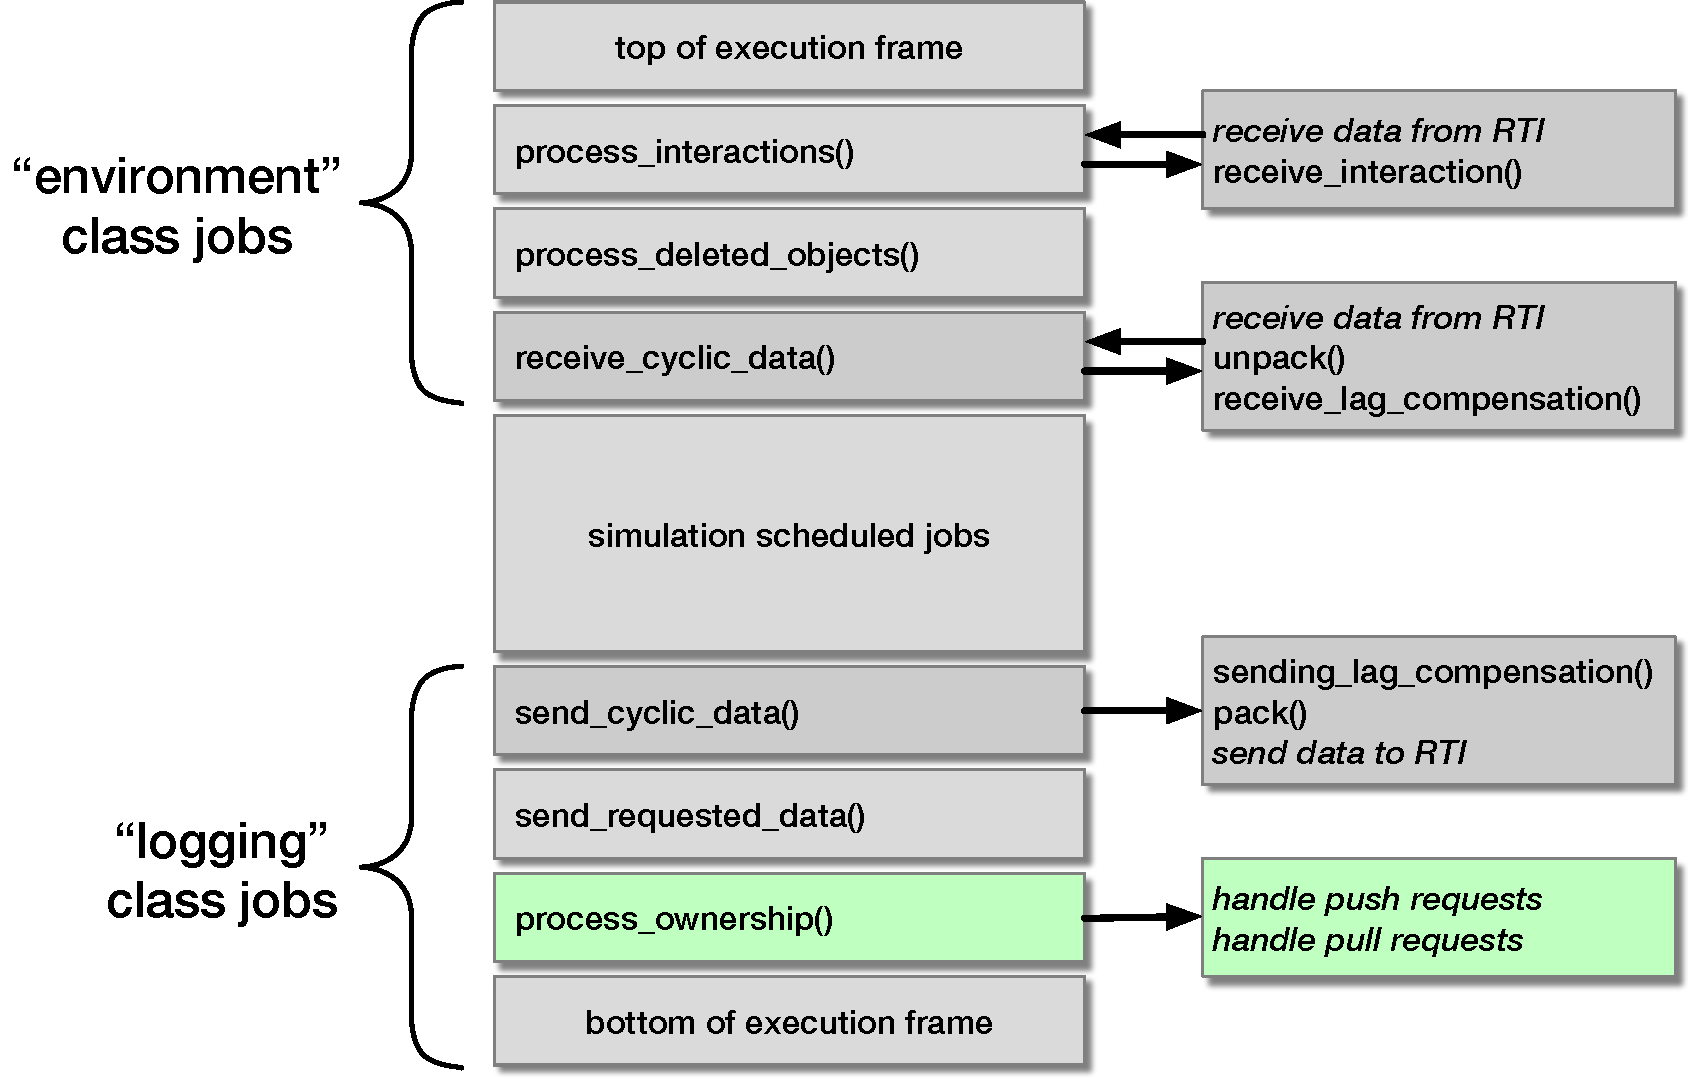
\includegraphics[scale=0.4]{TutorialTHLAOwnershipJobs.pdf}
      \end{figure}
   \end{frame}

   \begin{frame}
      \frametitle{Ownership Transfer}
      \framesubtitle{PITFALL - Handling Mixed Ownership}
      \begin{itemize}
         \item With ownership transfer, it is possible to have an object
         containing attributes you own and attributes you don’t own.
         \item TrickHLA knows to only send attributes you own, and only receive
         attributes you don’t own. However \ldots
         \item Your \texttt{unpack()} or \texttt{receive\_lag\_compensation()}
         functions run AFTER TrickHLA receives data, so they could accidently
         override your simulation state for attributes that you own and publish.
         This results in corrupted simulation data!
         \item To avoid overriding your simulation state, the solution is to
         determine if the attribute is owned by another federate in your
         \texttt{unpack()} and \texttt{receive\_lag\_compensation()} functions.
      \end{itemize}
      \begin{footnotesize}
      NOTE: the same scenario for your \texttt{pack()} or
      \texttt{send\_lag\_compensation()} functions is not a problem because
      they run BEFORE TrickHLA sends data, and because TrickHLA will not
      send data you don’t own, no harm done.
      \end{footnotesize}
         
   \end{frame}

   \begin{frame}[fragile]
      \frametitle{Ownership Transfer}
      \framesubtitle{PITFALL - Handling Mixed Ownership in Unpacking}
      \begin{itemize}
         \item Step 1: Add a \texttt{TrickHLA::Attribute} reference for each of
         your simulation state attributes. Example in \texttt{SinePacking.hh}:
      \end{itemize}
\begin{Verbatim}[frame=single, fontsize=\tiny]
   #include ”SineData.hh”
   #include "TrickHLA/include/TrickHLAAttribute.hh”
   #include "TrickHLA/include/TrickHLAPacking.hh”

   class SinePacking : public TrickHLAPacking
   {
     public:
      …
      // Initialize the packing object.
      void initialize( SineData * sim_data );
      // From the TrickHLAPacking class.
      virtual void initialize_callback( TrickHLAObject * obj );

      // From the TrickHLAPacking class.
      virtual void pack();
      // From the TrickHLAPacking class.
      virtual void unpack();

     private:
      SineData * sim_data; // -- Simulation data.
      double phase_deg;    // d  Phase offset in degrees.

      TrickHLAAttribute * phase_attr; // ** Reference to Phase TrickHLAAttribute.
   };
\end{Verbatim}
   \end{frame}

   \begin{frame}[fragile]
      \frametitle{Ownership Transfer}
      \framesubtitle{PITFALL - Handling Mixed Ownership in Unpacking (Continued)}
      \begin{itemize}
         \item Step 2: Override the \texttt{initialize\_callback()} function to
         set the attribute references.
         \item Example in \texttt{SinePacking.cpp}:
      \end{itemize}
\begin{Verbatim}[frame=single, fontsize=\scriptsize]
void SinePacking::initialize_callback( // RETURN: -- None.
   TrickHLAObject * obj ) // IN: -- Object associated with this packing class.
{
   // We must call the original function so that the callback is initialized.
   this->TrickHLAPacking::initialize_callback( obj );

   // Get a reference to the TrickHLAAttribute for the "Phase" FOM attribute.
   // We do this here so that we only do the attribute lookup once instead of
   // looking it up every time the unpack function is called.
   phase_attr = get_attribute_and_validate( "Phase" );
}
\end{Verbatim}
   \end{frame}

   \begin{frame}[fragile]
      \frametitle{Ownership Transfer}
      \framesubtitle{PITFALL - Handling Mixed Ownership in Unpacking (Continued)}
      \begin{itemize}
         \item Step 3: Check the attribute ownership in the unpack() function.
      \end{itemize}
\begin{Verbatim}[frame=single, fontsize=\scriptsize]
void SinePacking::unpack() // RETURN: -- None.
{
   // If the HLA phase attribute has changed and is remotely owned (i.e. is
   // coming from another federate) then override our simulation state with the
   // incoming value. If we locally own the "Phase" attribute then we do not
   // want to override it's value. If we did not do this check then we would be
   // overriding state of something we own and publish with whatever value
   // happen to be in the "phase_deg" local variable, which would cause data
   // corruption of the state. We always need to do this check because
   // ownership transfers could happen at any time or the data could be at a
   // different rate.
   if ( phase_attr->is_received() ) {
      // For this example to show how to use the Packing API's, we will
      // assume that the phase shared between federates is in degrees so
      // covert it back from degrees to radians.
      sim_data->set_phase( phase_deg * M_PI / 180.0 );
   }
}
\end{Verbatim}
   \end{frame}
   
